\documentclass[a4paper,10pt,twocolumn,english]{article}

% ============================================================================
% Packages
% ============================================================================

\usepackage{babel}
\usepackage[utf8]{inputenc}
\usepackage[T1]{fontenc}
\usepackage{lmodern}
\usepackage{amsmath,amssymb,amsthm,mathtools}
\usepackage{graphicx}
\usepackage{booktabs}
\usepackage{array}
\usepackage{tabularx}
\usepackage{longtable}
\usepackage{listings}
\usepackage{xcolor}
\usepackage{hyperref}
\usepackage{url}
\makeatletter
\g@addto@macro\UrlBreaks{\do\/\do\.\do\_\do\-\do\*}
\makeatother
\Urlmuskip=0mu\relax
\usepackage{enumitem}
\usepackage{microtype}
\usepackage{cleveref}
\usepackage[font=small,labelfont=bf]{caption}
\usepackage{float}
\usepackage{tikz}

% Reduce space between section number and title, prevent hyphenation in headings
\makeatletter
\renewcommand{\@seccntformat}[1]{\csname the#1\endcsname\hspace{0.5em}}
\renewcommand{\section}{\@startsection{section}{1}{\z@}%
  {-3.5ex \@plus -1ex \@minus -.2ex}%
  {2.3ex}%
  {\raggedright\normalfont\large\bfseries}}
\renewcommand{\subsection}{\@startsection{subsection}{2}{\z@}%
  {-3.25ex \@plus -1ex \@minus -.2ex}%
  {1.5ex}%
  {\raggedright\normalfont\normalsize\bfseries}}
\renewcommand{\subsubsection}{\@startsection{subsubsection}{3}{\z@}%
  {-3.25ex \@plus -1ex \@minus -.2ex}%
  {1.5ex}%
  {\raggedright\normalfont\small\bfseries}}
\makeatother
\usetikzlibrary{positioning,calc,arrows.meta}

% TikZ figure styles
\tikzset{
  figfont/.style={font=\scriptsize\sffamily},
  figbox/.style={draw, rounded corners=2pt, align=center, inner sep=4pt},
  figboxgray/.style={figbox, fill=gray!10},
  figsubbox/.style={figbox, fill=white},
  figsubboxgray/.style={figbox, fill=gray!5},
  figarrow/.style={-{Stealth[length=2mm]}, thick},
  figarrowstrong/.style={figarrow, line width=0.6pt},
}

% ============================================================================
% Typography improvements
% ============================================================================

\raggedbottom                           % Consistent local spacing
\widowpenalty=10000                     % Prevent widows (single lines at top)
\clubpenalty=10000                      % Prevent orphans (single lines at bottom)
\displaywidowpenalty=10000              % Prevent widows after display math
\predisplaypenalty=50                   % Discourage break before display math
\postdisplaypenalty=50                  % Discourage break after display math
\setlength{\emergencystretch}{2em}      % Reduce overfull lines in narrow columns
\setlength{\columnsep}{16pt}            % Slightly wider gutter for two-column reading
\setlength{\parskip}{0pt plus 1pt}      % Flexible paragraph spacing
\setlength{\floatsep}{10pt plus 2pt minus 2pt}
\setlength{\textfloatsep}{12pt plus 2pt minus 2pt}
\setlength{\intextsep}{10pt plus 2pt minus 2pt}
\setlength{\tabcolsep}{4pt}
\renewcommand{\arraystretch}{1.08}
\renewcommand{\topfraction}{0.85}       % Allow more floats at top
\renewcommand{\bottomfraction}{0.85}    % Allow more floats at bottom
\renewcommand{\textfraction}{0.10}      % Require less text on float pages
\renewcommand{\floatpagefraction}{0.7}  % Fuller float pages
\setcounter{topnumber}{2}
\setcounter{bottomnumber}{1}
\setcounter{totalnumber}{3}
\setlist[itemize]{leftmargin=*, itemsep=2pt, topsep=3pt}
\setlist[enumerate]{leftmargin=*, itemsep=2pt, topsep=3pt}
\setlist[description]{leftmargin=0pt, labelindent=0pt, itemsep=2pt, topsep=3pt}

% ============================================================================
% Numbering by section
% ============================================================================

\makeatletter
\@addtoreset{figure}{section}
\renewcommand{\thefigure}{\thesection.\arabic{figure}}
\@addtoreset{table}{section}
\renewcommand{\thetable}{\thesection.\arabic{table}}
\makeatother
\numberwithin{equation}{section}

% ============================================================================
% Theorem environments
% ============================================================================

\newtheoremstyle{paperplain}%
{3pt}{3pt}{\itshape\raggedright}{}{\bfseries}{}{0pt}%
{\thmname{#1}\thmnumber{ #2}\thmnote{. #3}.\hfill\break}
\newtheoremstyle{paperdef}%
{3pt}{3pt}{\normalfont\raggedright}{}{\bfseries}{}{0pt}%
{\thmname{#1}\thmnumber{ #2}\thmnote{. #3}.\hfill\break}
\newtheoremstyle{paperremark}%
{3pt}{3pt}{\normalfont\raggedright}{}{\itshape}{}{0pt}%
{\thmname{#1}\thmnumber{ #2}\thmnote{. #3}.\hfill\break}

\theoremstyle{paperdef}
\newtheorem{definition}{Definition}[section]

\theoremstyle{paperplain}
\newtheorem{theorem}[definition]{Theorem}
\newtheorem{lemma}[definition]{Lemma}
\newtheorem{proposition}[definition]{Proposition}
\newtheorem{corollary}[definition]{Corollary}

\theoremstyle{paperdef}
\newtheorem{example}[definition]{Example}
\newtheorem{assumption}{Assumption Block}[section]

\theoremstyle{paperremark}
\newtheorem{remark}[definition]{Remark}

% ============================================================================
% Custom commands
% ============================================================================

\newcolumntype{L}[1]{>{\raggedright\arraybackslash}p{#1}}
\newcommand{\thead}[1]{\textbf{\raisebox{0pt}[2.2ex][0.8ex]{#1}}}

\newcommand{\Coherent}{\ensuremath{\mathsf{Coherent}}}
\newcommand{\EdgeCoherent}{\ensuremath{\mathsf{EdgeCoherent}}}
\newcommand{\ActiveEdge}{\ensuremath{\mathsf{ActiveEdge}}}
\newcommand{\Consume}{\ensuremath{\mathsf{Consume}}}
\newcommand{\GEnv}{\ensuremath{\mathsf{GEnv}}}
\newcommand{\DEnv}{\ensuremath{\mathsf{DEnv}}}
\newcommand{\Hbyz}{\ensuremath{H_{\mathrm{byz}}}}
\newcommand{\Obssafe}{\ensuremath{\mathsf{Obs}_{\mathrm{safe}}^{\mathrm{byz}}}}
\newcommand{\Eqsafe}{\ensuremath{\mathsf{Eq}_{\mathrm{safe}}^{\mathrm{byz}}}}
\newcommand{\Ebyz}{\ensuremath{\mathcal{E}_{\mathrm{byz}}}}
\newcommand{\ByzSafe}{\ensuremath{\mathsf{ByzSafe}}}
\newcommand{\ByzChar}{\ensuremath{\mathsf{ByzChar}}}
\newcommand{\wf}{\ensuremath{\mathsf{wf}}}
\newcommand{\consumeOne}{\ensuremath{\mathsf{consumeOne}}}
\newcommand{\RecvCompatible}{\ensuremath{\mathsf{RecvCompatible}}}
\newcommand{\EdgeShares}{\ensuremath{\mathsf{EdgeShares}}}
\newcommand{\ByzIfaceWF}{\ensuremath{\mathsf{ByzIfaceWF}}}
\newcommand{\pathref}[1]{\texttt{#1}}
\newcommand{\eqnote}[1]{\par\noindent\textit{#1.}\par\vspace{-2pt}}

\newenvironment{citelist}{%
  \begin{list}{}{%
    \setlength{\leftmargin}{1.25em}%
    \setlength{\itemindent}{-1.25em}%
    \setlength{\itemsep}{2pt}%
    \setlength{\parsep}{0pt}%
    \setlength{\topsep}{3pt}}%
}{\end{list}}

\lstset{
  basicstyle=\ttfamily\footnotesize,
  keywordstyle=\color{blue},
  commentstyle=\color{gray},
  stringstyle=\color{red},
  breaklines=true,
  frame=leftline,
  rulecolor=\color{black!10},
  framerule=3pt,
  framesep=1em,
  columns=fullflexible,
  aboveskip=5pt,
  belowskip=5pt,
  xleftmargin=1.5em,
  literate={->}{$\to$\ }2 {forall}{$\forall$}1 {:=}{$\coloneqq$}2
}

% ============================================================================
% Document
% ============================================================================

\title{Coherence for Asynchronous Buffered MPST:\\A Mechanized Metatheory}
\author{S. H. Berman}
\date{\empty}

\begin{document}
\maketitle

\begin{abstract}
	Classical MPST uses coherence and projectability on global types to justify local safety. We define
	an operational coherence invariant, $\Coherent(G,D)$, over projected local environments and buffered
	traces, and show that this invariant is sufficient for preservation in asynchronous semantics. The
	operational coherence invariant yields a reusable three-way edge split that avoids per-step global
	re-derivation. Lean~4 mechanization confirms our results under parameterized delivery semantics.
\end{abstract}

% ============================================================================
\section{Introduction}
\label{sec:introduction}
% ============================================================================

\subsection{Background}

Multiparty session types guarantee that distributed protocols execute without communication errors.
The central technical challenge is preservation: showing that each protocol step maintains
well-typedness. Binary session types use duality to ensure two-party compatibility. MPST generalizes
this property by establishing global coherence and projectability conditions.

To address preservation, the MPST field has developed projection techniques that take a global
choreography to local session types. A global type specifies the full protocol, then projection
extracts the local view for each participant. Safety means that local executions remain consistent
with their projected types.

Classically, MPST coherence and projectability conditions are formulated at the global-type level (Honda,
Yoshida, and Carbone, 2008; Honda et al., 2016; Castagna et al., 2012), with later work
refining projection criteria (Majumdar et al., 2021).

In 2008, Honda et al.\ introduced asynchronous buffered MPST. Their preservation proof was organized
around global typing and projection consistency after transitions. Many later presentations keep this
global-first organization (Honda et al., 2016; Scalas and Yoshida, 2018), while
mechanized developments continue to refine proof organization and robustness (Tirore et al., 2025).

Prior MPST literature formulates coherence at the global-type level through projectability and
well-formedness conditions. This paper refines coherence at the operational level by using
$\Coherent(G,D)$ over local environments and buffered traces. Our operational formulation makes
preservation local and compositional and removes the long-standing per-step global re-derivation
bottleneck. We confirm this result via Lean 4 mechanization.

\subsection{Insight}

Projection defines a quotient, it erases global structure while preserving safety-relevant information.
The question is then: what exact invariant survives this erasure? We isolate an operational form of
coherence, $\Coherent(G,D)$, as the invariant required by our preservation proofs.
Binary session types use duality for two-party compatibility. This formulation instantiates n-ary
compatibility as receiver-buffer alignment at each active edge (Carbone et al., 2015).

$\Coherent(G,D)$ captures exactly what projection preserves for this proof architecture. It is
neither too strong nor too weak, and this exactness enables compositionality. Local proofs on individual
edges combine to yield global preservation. No global re-derivation is required.

\subsection{Technical Approach}

The core contribution is one operational kernel with two theorem-level lifts: typed-step preservation
and subtype replacement. The shared kernel is edge-local checking with active-edge lifting.
For typed transitions, this kernel is instantiated by a three-way edge split.
For subtype replacement, it is instantiated by \nolinkurl{Consume_mono} under receive-compatibility.

The local-to-global shape follows standard invariant methods from program logics (Reynolds, 2002;
O'Hearn, 2007), while aligning with process-calculus decomposition tradition (Plotkin, 1981;
Milner, 1999) and Lyapunov-style invariant-function reasoning in dynamical systems (Lyapunov, 1892;
LaSalle, 1960).

\begin{figure}[H]
	\centering
	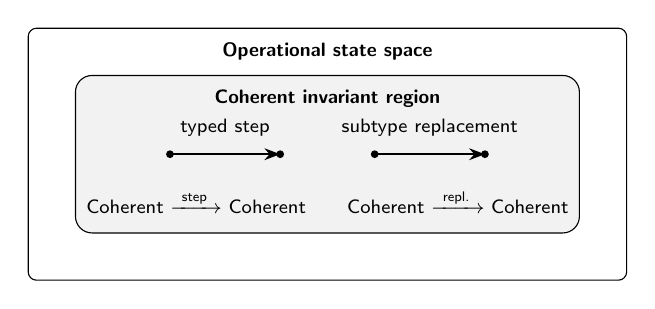
\begin{tikzpicture}[figfont, x=1mm, y=1mm]
		% State space boundary
		\draw[rounded corners=3pt] (-38,-14) rectangle (38,18);
		\node at (0,15) {\textbf{Operational state space}};

		% Coherent invariant region
		\draw[rounded corners=6pt, fill=gray!10] (-32,-8) rectangle (32,12);
		\node at (0,9) {\textbf{\textsf{Coherent} invariant region}};

		% Typed-step trajectory
		\fill (-20,2) circle (1.4pt);
		\fill (-6,2) circle (1.4pt);
		\draw[figarrowstrong] (-20,2) -- (-6,2);
		\node[anchor=south] at (-13,3) {typed step};

		% Subtype-replacement trajectory
		\fill (6,2) circle (1.4pt);
		\fill (20,2) circle (1.4pt);
		\draw[figarrowstrong] (6,2) -- (20,2);
		\node[anchor=south] at (13,3) {subtype replacement};

		% Symbolic statement
		\node[align=center] at (0,-4)
		{$\Coherent \xrightarrow{\;\text{step}\;} \Coherent
		\qquad
		\Coherent \xrightarrow{\;\text{repl.}\;} \Coherent$};
	\end{tikzpicture}
	\caption{Invariant-geometric view of preservation and subtype evolution.}
	\label{fig:p1-operational-kernel}
\end{figure}

\subsection{Scope and Claims}

This paper has two central claims. The first is Coherence preservation through a three-way split that
applies uniformly across transitions. The second is session evolution under subtype replacement via
\nolinkurl{Consume_mono}, which we lift to global Coherence and progress-condition preservation under
compatibility premises.

This paper starts a three-part series on asynchronous buffered semantics with
\texttt{DeliveryModel} parameterization. It precisely defines the invariant kernel.
\emph{Computable Dynamics for Asynchronous MPST} develops quantitative bounds and decision procedures on that kernel.
\emph{Harmony from Coherence in Asynchronous MPST} proves reconfiguration commutation and envelope exactness.

In this paper, our contributions are as follows:
\begin{enumerate}
	\item A mechanized operational Coherence architecture with a reusable three-way edge split and typed-step wrappers that lift edge-local lemmas to preservation and progress interfaces.
	\item A message-alignment proof kernel through \texttt{Consume} and the lemmas \nolinkurl{Consume_append} and \nolinkurl{Consume_cons}.
	\item A subtype-replacement theorem stack from \nolinkurl{Consume_mono} that preserves edge Coherence, global Coherence, and progress-side conditions under receive-compatibility premises.
	\item A delivery-parametric and premise-parametric typed effect bridge profile at the VM boundary.
\end{enumerate}

\begin{center}
	\small
			\begin{tabularx}{\columnwidth}{@{}L{0.36\columnwidth}L{0.59\columnwidth}@{}}
			\toprule
			\thead{Symbol} & \thead{Meaning}                     \\
			\midrule
			$\Hbyz$         & Byzantine characterization bundle    \\
			$\Obssafe$      & Byzantine safety-visible observation \\
			$\Eqsafe$       & Byzantine safety-visible equality    \\
				$\Ebyz$         & Byzantine determinism-envelope       \\
				$\ByzChar$      & Byzantine characterization formula    \\
				$\ByzSafe$      & Byzantine safety predicate            \\
				\ByzIfaceWF     & Byzantine interface well-formedness   \\
				\Coherent       & global active-edge compatibility     \\
				\EdgeCoherent   & edge-local compatibility check       \\
				\EdgeShares     & edge-to-endpoint incidence predicate \\
				\Consume        & trace-to-type alignment function     \\
				\GEnv           & endpoint-to-local-type environment    \\
				\DEnv           & edge-to-buffered-trace environment    \\
			\ActiveEdge     & endpoint-presence guard              \\
			\RecvCompatible & receive-side replacement compatibility \\
			\texttt{DeliveryModel} & parametric delivery interface \\
			\bottomrule
		\end{tabularx}
	\captionof{table}{Notation used in this paper.}
\end{center}

% ============================================================================
\section{Model and Semantics}
\label{sec:model}
% ============================================================================

Configurations are represented by endpoint and edge environments. \GEnv{} maps endpoints to local types. \DEnv{} maps directed edges to buffered type traces. \texttt{Buffers} maps directed edges to runtime payload queues.

\begin{table}[H]
	\centering
	\small
	\begin{tabularx}{\columnwidth}{@{}L{0.55\columnwidth}L{0.4\columnwidth}@{}}
		\toprule
		\thead{Assumption}             & \thead{Status}      \\
		\midrule
		asynchronous buffered semantics & required             \\
		active-edge quantification      & required             \\
		fair scheduling profile         & assumed where stated \\
		\texttt{DeliveryModel} param.   & required             \\
		crash-stop and Byzantine claims & interface claim only \\
		\bottomrule
	\end{tabularx}
	\caption{Model assumptions for exact statements in this paper.}
\end{table}

\begin{assumption}[Core Model Premises]
	\label{assump:p1-core}
	Core claims in this paper assume asynchronous buffered semantics, active-edge quantification, and \texttt{DeliveryModel} parameterization. Fair scheduling assumptions apply where stated.
\end{assumption}

\begin{definition}[Active Edge]
	$\ActiveEdge(G, e)$ holds when both endpoints of edge $e$ are present in $G$.
\end{definition}

\begin{definition}[Edge Coherence]
	$\EdgeCoherent(G, D, e)$ holds when the receiver side can consume the buffered trace on edge $e$ under the local type in $G$.
\end{definition}

\begin{definition}[Coherence]
	$\Coherent(G, D)$ holds when every active edge is edge coherent.
\end{definition}

\begin{definition}[Consume]
	$\Consume$ is the recursive alignment function that interprets buffered traces against receiver expectations.
\end{definition}

\begin{definition}[Byzantine Interface Well-Formedness]
	$\ByzIfaceWF(G, D)$ is the interface predicate used for Byzantine-facing statements in this paper, and is mechanized as a definitional alias of $\Coherent(G, D)$.
\end{definition}

Delivery behavior is parameterized by \texttt{DeliveryModel}. This gives one theorem shape across FIFO, causal, and lossy instances.
\begin{equation}
	\label{eq:p1-active-edge-boundary}
	\begin{aligned}[t]
		\Coherent(G,D)\ :=\ \forall e,\ \ActiveEdge(G,e)
		\\
		\to\ \EdgeCoherent(G,D,e).
	\end{aligned}
\end{equation}
Edges incident to absent endpoints are excluded by $\ActiveEdge$.

\subsection{Why Coherence}

The term follows the linear-logic compatibility tradition from coherence-space semantics and session typing foundations, including Girard (1987), Caires and Pfenning (2010), and Wadler (2012). Usage in this paper is operational rather than denotational.

This operational usage is aligned with, but distinct from, classical MPST global coherence and projectability (Honda et al., 2008; Honda et al., 2016; Castagna et al., 2012) and logical n-ary coherence accounts (Carbone et al., 2015; Carbone et al., 2016; Carbone et al., 2017).

Operationally, our edge-local notion also sits in the lineage connecting session typing, subtyping, and communicating-automata views (Gay and Hole, 2005; Deni\'{e}lou and Yoshida, 2012; Brand and Zafiropulo, 1983).

The key structural correspondence is compatibility. A coherence-space token corresponds to an edge-local communication view, and a clique corresponds to a globally coherent configuration over active edges.

\begin{table}[H]
	\centering
	\small
	\begin{tabularx}{\columnwidth}{@{}L{0.38\columnwidth}L{0.57\columnwidth}@{}}
		\toprule
		\thead{Coherence-space} & \thead{MPST operational}         \\
		\midrule
		token                    & directed edge with buffered trace \\
		coherence relation       & \texttt{EdgeCoherent}             \\
		clique                   & \texttt{Coherent} configuration   \\
		linear-map preservation  & step preservation theorem         \\
		\bottomrule
	\end{tabularx}
	\caption{Coherence-space correspondence.}
\end{table}

% ============================================================================
\section{Worked Example}
\label{sec:example}
% ============================================================================

\noindent\begingroup\raggedright
\textbf{Running example.} Roles are \texttt{C} (client), \texttt{P} (pool), and \texttt{M} (monitor), with global interaction:
\par\endgroup

\noindent\begin{minipage}{\columnwidth}
	\begin{lstlisting}
C -> P : Request(n)
P -> C : Grant(k)
C -> M : Report(k)
M -> P : Confirm
P -> C : Token(t)
\end{lstlisting}
\end{minipage}

Fix local continuations:

\noindent\begin{minipage}{\columnwidth}
	\begin{lstlisting}
L_C := recv P Grant(k);
       send M Report(k);
       recv P Token(t); end
L_P := recv M Confirm;
       send C Token(t); end
L_M := recv C Report(k);
       send P Confirm; end
\end{lstlisting}
\end{minipage}

and in-flight configuration $(G_0,D_0)$:

\noindent\begin{minipage}{\columnwidth}
	\begin{lstlisting}
G_0(C) = L_C
G_0(P) = L_P
G_0(M) = L_M
D_0(P,C) = [Grant(k)]
D_0(e)   = []    for e != (P,C)
\end{lstlisting}
\end{minipage}

Assume typing judgment $\Gamma \vdash (G_0,D_0)\ \wf$.

The active-edge obligation is:
\begin{equation}
	\forall e,\ \ActiveEdge(G_0,e)\to \EdgeCoherent(G_0,D_0,e).
\end{equation}
The example is used via the following derived rule instances.

		{\footnotesize
			\begin{gather}
				\dfrac{
					\Gamma \vdash (G_0,D_0)\ \wf \quad D_0(P,C){=}[\mathrm{Grant}(k)]
				}{
					(G_0,D_0){\to}(G_1,D_1) \land \Coherent(G_1,D_1)
				}\hspace{0.75em}
				\\[10pt]
				\dfrac{
					\Gamma \vdash (G_1,D_1)\ \wf \quad \mathsf{Consume\_append}
				}{
					(G_1,D_1){\to}(G_2,D_2) \land \Coherent(G_2,D_2)
				}\hspace{0.75em}
				\\[10pt]
				\dfrac{
					\Coherent(G_0,D_0) \quad \RecvCompatible(G_0,G'_0)
			}{
				\Coherent(G'_0,D_0)
			}\hspace{0.75em}
		\end{gather}
		\vspace{6pt}
	}

For the step edge $u=(C,M)$ with stepped endpoint $ep_{\mathrm{step}}$, the case split used later is: updated ($e=u$), shared-endpoint ($e\neq u \land \EdgeShares(e,ep_{\mathrm{step}})$), and unrelated ($e\neq u \land \neg\EdgeShares(e,ep_{\mathrm{step}})$).

% ============================================================================
\section{Coherence Preservation Architecture}
\label{sec:preservation}
% ============================================================================

\begin{figure}[H]
	\centering
	\resizebox{\columnwidth}{!}{%
		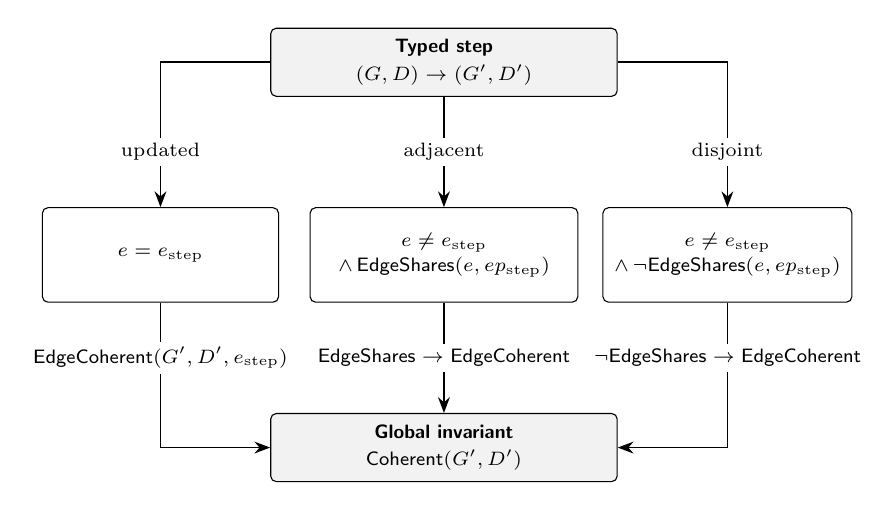
\begin{tikzpicture}[figfont]
			% Typed step at top
			\node[figboxgray, minimum width=44mm] (step)
			{\textbf{Typed step}\\[2pt] $(G,D)\to(G',D')$};

			% Three-way split: predicate boxes only (case names on arrows)
			\node[figsubbox, below=14mm of step, xshift=-36mm, minimum width=30mm, minimum height=12mm] (updated)
			{$e=e_{\mathrm{step}}$};
			\node[figsubbox, below=14mm of step, minimum width=34mm, minimum height=12mm] (shared)
			{$e\neq e_{\mathrm{step}}$\\[1pt] $\land\,\EdgeShares(e,ep_{\mathrm{step}})$};
			\node[figsubbox, below=14mm of step, xshift=36mm, minimum width=30mm, minimum height=12mm] (unrel)
			{$e\neq e_{\mathrm{step}}$\\[1pt] $\land\,\neg\EdgeShares(e,ep_{\mathrm{step}})$};

			\node[figboxgray, below=14mm of shared, minimum width=44mm] (global)
			{\textbf{Global invariant}\\[2pt] $\Coherent(G',D')$};

			% Labeled arrows from step to each case
			\draw[figarrowstrong] (step) -- (shared);
			\draw[figarrowstrong] (step.west) -- (updated.north |- step.west) -- (updated.north);
			\draw[figarrowstrong] (step.east) -- (unrel.north |- step.east) -- (unrel.north);
			\coordinate (label-y-top) at ($(step.south)!0.5!(shared.north)$);
			\node[font=\scriptsize, fill=white, inner sep=2pt] at (updated |- label-y-top) {updated};
			\node[font=\scriptsize, fill=white, inner sep=2pt] at (shared |- label-y-top) {adjacent};
			\node[font=\scriptsize, fill=white, inner sep=2pt] at (unrel |- label-y-top) {disjoint};

			% Labeled arrows from cases to global invariant
			\draw[figarrowstrong] (updated.south) |- (global.west);
			\draw[figarrowstrong] (shared.south) -- (global.north);
			\draw[figarrowstrong] (unrel.south) |- (global.east);
			\coordinate (label-y-bot) at ($(shared.south)!0.5!(global.north)$);
			\node[font=\scriptsize, fill=white, inner sep=2pt] at (updated |- label-y-bot) {$\EdgeCoherent(G',D',e_{\mathrm{step}})$};
			\node[font=\scriptsize, fill=white, inner sep=2pt] at (shared |- label-y-bot) {$\EdgeShares \to \EdgeCoherent$};
			\node[font=\scriptsize, fill=white, inner sep=2pt] at (unrel |- label-y-bot) {$\neg\EdgeShares \to \EdgeCoherent$};
		\end{tikzpicture}
	}%
	\caption{Three-way edge split used by the preservation proof.}
	\label{fig:p1-preservation-architecture}
\end{figure}

\begin{theorem}[Coherence Preservation]
	\label{thm:coherence-preservation}
	For all environments $G,D,G',D'$, if $(G,D) \to (G',D')$ is a well-typed step in the send and recv and select and branch fragment, then
	\begin{equation}
		\Coherent(G,D) \implies \Coherent(G',D').
	\end{equation}
	This claim is exact for one-step preservation in the stated core rule fragment.
\end{theorem}

\begin{proof}[Proof sketch]
	The argument is a reusable case-analysis pipeline over edges.

	\begin{enumerate}
		\item Fix a typed one-step transition and an arbitrary edge $e$ that is active after the step.
		\item Apply \nolinkurl{edge_case_split} to partition $e$ into:
		      \begin{itemize}
			      \item updated edge ($e = e_{\mathrm{step}}$),
			      \item shared-endpoint edge ($e \neq e_{\mathrm{step}} \land \EdgeShares(e, ep_{\mathrm{step}})$),
			      \item unrelated edge ($e \neq e_{\mathrm{step}} \land \neg \EdgeShares(e, ep_{\mathrm{step}})$).
		      \end{itemize}
		\item Updated-edge case: send/recv/select/branch obligations are discharged by rule-local preservation lemmas; message-to-type alignment is reduced to \nolinkurl{Consume_append} (enqueue-facing) or \nolinkurl{Consume_cons} (dequeue-facing).
		\item Shared-endpoint case: use store/buffer irrelevance lemmas to show unaffected projections are preserved; transport pre-state $\EdgeCoherent$ to post-state $\EdgeCoherent$.
		\item Unrelated-edge case: apply frame-style transport (no touched endpoint, no touched buffer segment); conclude edge-local coherence is unchanged.
		\item Reassemble all cases to obtain $\Coherent(G',D')$.
	\end{enumerate}

	The same skeleton is used uniformly across send/recv/select/branch, which is the main proof-reuse gain in this paper.
\end{proof}

The split operator is implemented by \nolinkurl{edge_case_split}. Rule-level preservation lemmas are grouped by send, recv, select, and branch cases. Table~\ref{tab:p1-claim-artifact-map} gives the primary module map, and \cref{app:chains} records theorem-to-lemma chains with exact Lean anchors.

The architecture is quotient-first. The concrete step relation induces dynamics on equivalence classes once coherence-preserving symmetries are quotiented out.

The quotienting step should be read as symmetry reduction. Distinct interleavings that are equivalent under the symmetry relation are identified as one observable class. Formally, the induced square is:
\begin{equation}
	q(\mathsf{step}(C))\ =\ \mathsf{step}_{/ \sim}(q(C)).
\end{equation}
The square states the commuting condition used across these three papers. This paper establishes the preservation side needed to make the quotient dynamics well-defined.

The case partition used by \nolinkurl{edge_case_split} is:
\eqnote{Case partition for checked edge}
Here $S(e):=\EdgeShares(e,ep_{\mathrm{step}})$.
\begin{equation}
	\begin{aligned}
		\mathsf{updated}   & :\ e=u;\\
		\mathsf{shared}    & :\ e\neq u\land S(e);\\
		\mathsf{unrelated} & :\ e\neq u\land \neg S(e).
	\end{aligned}
\end{equation}
The three branches are discharged by updated-edge preservation, shared-endpoint transport, and unrelated-edge frame transport, respectively.

% ============================================================================
\section{Message-Type Alignment via Consume}
\label{sec:consume}
% ============================================================================

$\Consume$ is the proof kernel for message-type alignment. It removes most rule-specific structural complexity from preservation proofs.

\begin{lemma}[Consume\_append]
	Consumption over concatenated traces factors through sequential consumption.
\end{lemma}

\begin{lemma}[Consume\_cons]
	Head consumption reduces to one-step alignment plus recursive continuation alignment.
\end{lemma}

\begin{proof}[Proof sketch]
	The library is centered on $\consumeOne$ and structural recursion on trace shape.

	\begin{enumerate}
		\item \nolinkurl{Consume_append}: induction on trace prefix $ts$; base case $ts = []$ is immediate by simplification ($L' = L_r$); step case peels one $\consumeOne$ transition and applies induction hypothesis to the residual local type.
		\item \nolinkurl{Consume_cons}: unfold one $\Consume$ step on head $T$; case split on $\consumeOne(\mathit{from}, T, L_r)$; resulting equation is definitional in both branches.
		\item Preservation integration: send/select proofs use \nolinkurl{Consume_append} to justify extending buffered traces; recv/branch proofs use \nolinkurl{Consume_cons} to justify consuming the head message and continuing.
	\end{enumerate}

	This isolates alignment complexity into two reusable lemmas rather than duplicating ad-hoc trace reasoning in each operational rule.
\end{proof}

For the worked example, \nolinkurl{Consume_cons} discharges the \texttt{Grant} receive step at \texttt{C} by reducing the obligation to continuation coherence after one aligned message.

% ============================================================================
\section{Session Evolution via Subtyping}
\label{sec:evolution}
% ============================================================================

Session evolution replaces one endpoint local type with a compatible refinement and asks whether coherence is preserved.

This replacement argument follows a standard commutation intuition from trace-equivalence and commuting-conversion lines. The standard point is that local reorderings or local refinements should preserve observable behavior when compatibility conditions hold. What is new here is an operational criterion for asynchronous subtype replacement that is stated directly through \nolinkurl{Consume_mono} and discharged with edge-local coherence obligations.

\begin{assumption}[Replacement Compatibility]
	\label{assump:p1-replacement}
	The subtype-evolution theorem assumes endpoint replacement at $ep$ satisfies typing-domain preservation, receive-side monotonicity side conditions, and environment consistency for unaffected endpoints.
\end{assumption}

\begin{theorem}[Session Evolution via \nolinkurl{Consume_mono}]
	\label{thm:session-evolution}
	For all endpoints $ep$ and environments $G,D,G_{\mathrm{rep}}$, if Assumption Block~\ref{assump:p1-replacement} holds for replacement at $ep$, then
	\begin{equation}
		\Coherent(G,D) \implies \Coherent(G_{\mathrm{rep}},D).
	\end{equation}
	This claim is exact for type replacement steps covered by Assumption Block~\ref{assump:p1-replacement}.
\end{theorem}

\begin{proof}[Proof sketch]
	The replacement theorem is proved by a monotonicity-to-global-lift chain.

	\begin{enumerate}
		\item Local monotonicity: establish receive-compatibility ($\RecvCompatible$) between old and replacement local types; apply \nolinkurl{Consume_mono} to show every successful old consumption remains successful after replacement.
		\item Edge lift: use \nolinkurl{EdgeCoherent_type_replacement} on edges targeting the replaced endpoint; for non-target edges, transport coherence by environment agreement.
		\item Global lift: combine edge cases to derive \nolinkurl{Coherent_type_replacement}.
		\item Progress compatibility: use liveness-side lemmas (\nolinkurl{progress_conditions_type_replacement}) to preserve operational side conditions.
	\end{enumerate}

	Hence compatible subtype replacement preserves Coherence without re-running global derivations.
\end{proof}

Core lemmas are in the subtype-replacement core and liveness layers.
The subtype-replacement commutation principle and proof-lift chain are:
\begin{equation}
	\begin{aligned}[t]
		\Coherent(G,D)\ \land\ \mathsf{Compat}_{ep}(G,G_{\mathrm{rep}})
		\\
		\Longrightarrow\ \Coherent(G_{\mathrm{rep}},D).
	\end{aligned}
\end{equation}
\begin{equation}
	\texttt{Consume\_mono}\ \Longrightarrow\ \text{edge lift}\ \Longrightarrow\ \text{global lift}.
\end{equation}
with compatibility discharged by \nolinkurl{Consume_mono} and replacement side conditions.

% ============================================================================
\section{Mechanization Summary}
\label{sec:mechanization}
% ============================================================================

Table~\ref{tab:p1-claim-artifact-map} maps each core claim to concrete modules and representative theorem anchors.
Module references use path identifiers of the form \texttt{P$n$-A$xx$}, where $n$ is the paper number and $xx$ is the artifact index; these resolve to file paths in Appendix~\ref{app:p1-path-registry}.

\begin{table}[H]
	\centering
	\footnotesize
			\begin{tabularx}{\columnwidth}{@{}L{0.23\columnwidth}L{0.28\columnwidth}L{0.41\columnwidth}@{}}
			\toprule
			\thead{Claim}    & \thead{Modules}                              & \thead{Anchors}                        \\
			\midrule
			Definitions       & \pathref{P1-A01},\allowbreak \pathref{P1-A02} & \texttt{Consume}, \texttt{EdgeCoherent},\allowbreak\ \texttt{Coherent} \\
			Consume kernel    & \pathref{P1-A01}                              & \nolinkurl{Consume_append}              \\
			Three-way split   & \pathref{P1-A03}                              & \nolinkurl{edge_case_split}             \\
			Preservation      & \pathref{P1-A04},\allowbreak \pathref{P1-A07},\allowbreak \pathref{P1-A08} & \nolinkurl{Coherent_send_preserved},\allowbreak\ \nolinkurl{Coherent_recv_preserved},\allowbreak\ \nolinkurl{Coherent_select_preserved},\allowbreak\ \nolinkurl{Coherent_branch_preserved} \\
			Delivery variants & \pathref{P1-A05}                              & \nolinkurl{FIFODelivery_laws},\allowbreak\ \nolinkurl{CausalDelivery_laws},\allowbreak\ \nolinkurl{LossyDelivery_laws}              \\
			Subtype repl.     & \pathref{P1-A06}                              & \nolinkurl{Consume_mono},\allowbreak\ \nolinkurl{Coherent_type_replacement},\allowbreak\ \nolinkurl{progress_conditions_type_replacement}                \\
			\bottomrule
		\end{tabularx}
	\caption{Claim to artifact mapping.}
	\label{tab:p1-claim-artifact-map}
\end{table}

% ============================================================================
\section{Effect-Typed Bridge}
\label{sec:bridge}
% ============================================================================

\texttt{EffectSpec.handlerType} records typed effect obligations at the VM boundary. Bridge results in
this section are conditional on explicit monitor and quotient-transport premises.

\begin{proposition}[Bridge Soundness]
	For any selected handler $h$, if choreography obligations for $h$ are discharged, \texttt{EffectSpec.handlerType} holds for $h$, \nolinkurl{monitor_sound} and \nolinkurl{unified_monitor_preserves} hold for the active monitor, and the configuration-equivalence/effect-bisimulation bridge assumptions hold, then VM-side typing obligations generated from $h$ are satisfied in the corresponding runtime instruction layer and transport to the observational interface.
\end{proposition}

\begin{proof}[Proof sketch]
	Build the bundled bridge premises \texttt{VMBridgePremises} from \nolinkurl{monitor_sound},\allowbreak\ \nolinkurl{unified_monitor_preserves}, and the \nolinkurl{WellTypedInstr.wt_invoke} handler-typing witness. Lift handler typing from local obligations to short instruction fragments and then to VM-step form through \nolinkurl{handler_obligation_local},\allowbreak\ \nolinkurl{handler_fragment_typing_of_premises}, and \nolinkurl{handler_vm_step_typing}. Compose with \nolinkurl{configEquiv_iff_effectBisim_silent} and \nolinkurl{effectBisim_implies_observationalEquivalence} via \nolinkurl{vm_bridge_soundness_composed}. Therefore the runtime typing obligations and their observational transport both follow under the stated premises.
\end{proof}

\begin{table}[H]
	\centering
	\small
	\begin{tabularx}{\columnwidth}{@{}L{0.45\columnwidth}L{0.5\columnwidth}@{}}
		\toprule
		\thead{Bridge item}    & \thead{Role}               \\
		\midrule
		choreography obligation & source protocol obligation  \\
		effect handler typing   & typed executable obligation \\
		VM runtime typing check & enforcement layer           \\
		\bottomrule
	\end{tabularx}
	\caption{Bridge intent.}
\end{table}

\begin{assumption}[Byzantine Interface Premises]
	\label{assump:p1-byzantine}
	The interface statements in this section assume shared notation for $\Hbyz$, $\Obssafe$, $\Eqsafe$, and $\Ebyz$, plus theorem-pack capability naming consistency between abstract and runtime layers.
\end{assumption}

\begin{theorem}[Byzantine Interface Well-Formedness (BZ-1)]
	Under Assumption Block~\ref{assump:p1-byzantine}, Byzantine safety-track statements in this paper are interpreted on configurations $(G,D)$ satisfying $\ByzIfaceWF(G,D)$ (definitional alias of $\Coherent(G,D)$). For any active edge, this interface yields the same sender-existence and $\Consume$ obligations as the Coherence layer.
\end{theorem}

\begin{corollary}[Dropped-Assumption Witness Interface (BZ-1.1)]
	Let $\mathcal{A}$ be any assumption class named in $\Hbyz$. If a later construction provides a witness violating $\ByzSafe$ when $\mathcal{A}$ is dropped, then that witness can be expressed against the same active-edge Coherence interface used in this paper.
\end{corollary}

\begin{proposition}[Capability-Gated VM Interface (BZ-1.2)]
	If a runtime profile includes Byzantine characterization and envelope-adherence capability evidence, then safety-visible runtime obligations are interpreted through $\Eqsafe$ modulo $\Ebyz$, and profile admission is blocked when required evidence is absent.
\end{proposition}

% ============================================================================
\section{Related Work}
\label{sec:related}
% ============================================================================

Classical MPST establishes global coherence and projectability as conditions on global types and projection (Honda et al., 2008, Honda et al., 2016, Castagna et al., 2012, and Majumdar et al., 2021). Logical lines interpret multiparty compatibility as n-ary duality and proof compatibility (Carbone et al., 2015, Carbone et al., 2016, and Carbone et al., 2017). Data certification extensions remain in the same global-projection discipline (Toninho and Yoshida, 2017).

This paper refines the established notion of coherence in MPST with an operational invariant $\Coherent(G,D)$ over local environments and buffered traces. The novelty is an asynchronous preservation architecture that discharges obligations edge-locally and avoids per-step global re-derivation.

Local-first and rely/guarantee lines motivate alternatives to global-first checks (Scalas and Yoshida, 2018). Program-logical lines such as Actris target implementation proofs over protocol resources at a different verification layer (Hinrichsen et al., 2020). Event-structure and partial-order lines provide complementary macro semantics for concurrency (Castellan et al., 2023).

Compared with these lines, this paper contributes a reusable proof kernel that combines a three-way edge split, \texttt{Consume}-based message alignment, subtype-replacement monotonicity, and delivery-parametric preservation under explicit premises. It also gives a premise-conditional VM bridge chain that composes monitor contracts with effect-bisimulation transport.

\begin{table}[H]
	\centering
	\small
	\begin{tabularx}{\columnwidth}{@{}L{0.47\columnwidth}L{0.48\columnwidth}@{}}
		\toprule
		\thead{Prior limitation}                 & \thead{Contribution}                    \\
		\midrule
		preservation tied to global re-derivation & reusable edge-local skeleton             \\
		weak theory/execution boundary            & explicit effect-typed bridge             \\
		FIFO-centric semantics                    & one theorem under \texttt{DeliveryModel} \\
		fragmented proof structure                & split kernel + \texttt{Consume} lemmas   \\
		\bottomrule
	\end{tabularx}
	\caption{Comparison with prior work.}
\end{table}

% ============================================================================
\section{Limitations and Scope}
\label{sec:limitations}
% ============================================================================

This paper proves preservation and progress for the typed asynchronous core rule family through the
operational Coherence architecture. It also proves subtype replacement stability for edge Coherence,
global Coherence, and progress-side conditions when replacement preserves typing domains, satisfies
receive-side monotonicity, and keeps unaffected endpoints environment-consistent. VM bridge claims are
conditional on explicit monitor and quotient-transport premises rather than unconditional runtime
metatheorems.

Quantitative, fault-characterization, and envelope-level claims are proved in later papers within this series.

% ============================================================================
\section{Conclusion}
\label{sec:conclusion}
% ============================================================================

Since Honda et al.\ (2008), many preservation accounts for asynchronous MPST have been organized around global re-derivation after each step. This paper provides a mechanized alternative.

The key insight is that projection from global to local types defines an erasure. The operational invariant $\Coherent(G,D)$ is exact for our preservation architecture. Because it is exact at the operational boundary, local proofs compose without global re-derivation.

The resulting kernel is small, compositional, and extensible. It supports subtype-driven session evolution through a single monotonicity lemma. The mechanization in Lean~4 confirms that the architecture scales.

% ============================================================================
\section*{Works Cited}
% ============================================================================

\begin{citelist}
	\item Baier, C., and Katoen, J.-P. (2008). Principles of Model Checking. MIT Press.
	\item Brand, D., and Zafiropulo, P. (1983). On Communicating Finite-State Machines. Journal of the ACM, 30(2), 323--342.
	\item Caires, L., and Pfenning, F. (2010). Session Types as Intuitionistic Linear Propositions. CONCUR 2010.
	\item Carbone, M., Lindley, S., Montesi, F., Sch\"urmann, C., and Wadler, P. (2016). Coherence Generalises Duality: A Logical Explanation of Multiparty Session Types. CONCUR 2016.
	\item Carbone, M., Montesi, F., Sch\"urmann, C., and Yoshida, N. (2015). Multiparty Session Types as Coherence Proofs. CONCUR 2015.
	\item Carbone, M., Montesi, F., Sch\"urmann, C., and Yoshida, N. (2017). Multiparty Session Types as Coherence Proofs. Acta Informatica, 54(3), 243--269.
	\item Castagna, G., Dezani-Ciancaglini, M., Gesbert, N., and Padovani, L. (2012). On Global Types and Multi-Party Sessions.
	\item Castellan, S., et al. (2023). Event-structure and partial-order semantics for session-based concurrency. Journal of Logic and Algebraic Methods in Programming.
	\item Cover, T. M., and Thomas, J. A. (2006). Elements of Information Theory (2nd ed.). Wiley.
	\item Deni\'{e}lou, P.-M., and Yoshida, N. (2012). Multiparty Session Types Meet Communicating Automata. ESOP 2012.
	\item Gay, S. J., and Hole, M. (2005). Subtyping for Session Types in the Pi Calculus. Acta Informatica, 42(2--3), 191--225.
	\item Girard, J.-Y. (1987). Linear Logic. Theoretical Computer Science, 50(1), 1--101.
	\item Hinrichsen, J., et al. (2020). Actris: Session-type based reasoning in separation logic. POPL 2020.
	\item Hoare, C. A. R. (1985). Communicating Sequential Processes. Prentice Hall.
	\item Honda, K. (1993). Types for Dyadic Interaction. CONCUR 1993.
	\item Honda, K., Vasconcelos, V. T., and Kubo, M. (1998). Language Primitives and Type Discipline for Structured Communication-Based Programming. ESOP 1998.
	\item Honda, K., Yoshida, N., and Carbone, M. (2008). Multiparty Asynchronous Session Types. POPL 2008.
	\item Honda, K., Yoshida, N., and Carbone, M. (2016). Multiparty Asynchronous Session Types. Journal of the ACM, 63(1), Article 9.
	\item LaSalle, J. P. (1960). Some Extensions of Liapunov's Second Method. IRE Transactions on Circuit Theory, 7(4), 520--527.
	\item Lyapunov, A. M. (1892). The General Problem of the Stability of Motion. Kharkov Mathematical Society.
	\item Majumdar, R., Mukund, M., Stutz, F., and Zufferey, D. (2021). Generalising Projection in Asynchronous Multiparty Session Types. CONCUR 2021.
	\item Milner, R. (1999). Communicating and Mobile Systems: The Pi-Calculus. Cambridge University Press.
	\item Milner, R., Parrow, J., and Walker, D. (1992). A Calculus of Mobile Processes, I and II. Information and Computation, 100(1), 1--77.
	\item O'Hearn, P. W. (2007). Resources, Concurrency, and Local Reasoning. Theoretical Computer Science, 375(1--3), 271--307.
	\item Pierce, B. C. (2002). Types and Programming Languages. MIT Press.
	\item Plotkin, G. D. (1981). A Structural Approach to Operational Semantics. DAIMI FN-19.
	\item Reynolds, J. C. (2002). Separation Logic: A Logic for Shared Mutable Data Structures. LICS 2002.
	\item Scalas, A., and Yoshida, N. (2018). Multiparty Session Types, Beyond Duality. Journal of Logical and Algebraic Methods in Programming, 97, 55--84.
	\item Shannon, C. E. (1948). A Mathematical Theory of Communication. Bell System Technical Journal, 27(3), 379--423 and 27(4), 623--656.
	\item Tirore, L., Bengtson, J., and Carbone, M. (2025). Mechanized MPST metatheory with subject-reduction robustness analysis. ECOOP 2025.
	\item Toninho, B., and Yoshida, N. (2017). Certifying Data in Multiparty Session Types. Journal of Logical and Algebraic Methods in Programming, 90, 61--83.
	\item Wadler, P. (2012). Propositions as Sessions. ICFP 2012.
\end{citelist}

% ============================================================================
\clearpage
\appendix
\noindent{\Large\bfseries Appendix}
\vspace{0.5em}
% ============================================================================

\section{Syntax and Judgments}
\label{app:syntax}

This appendix fixes the formal objects and judgment forms used in Sections~2--6.

\subsection{Roles, Endpoints, and Edges}

Let \texttt{Role} be the finite set of role names. An endpoint is a pair $(\mathit{sid},r)$ of session identifier and role. A directed edge is a triple $(\mathit{sid}, r_s, r_r)$ with sender role $r_s$ and receiver role $r_r$.

We write:
\begin{itemize}
	\item $\mathsf{src}(e)$ for the sender endpoint of edge $e$,
	\item $\mathsf{dst}(e)$ for the receiver endpoint of edge $e$,
	\item $\mathsf{role}(ep)$ for the role component of endpoint $ep$,
	\item $\EdgeShares(e, ep)$ when endpoint $ep$ is either $\mathsf{src}(e)$ or $\mathsf{dst}(e)$.
\end{itemize}

\subsection{Local Types and Environments}

Local types are generated by:

\noindent\begin{minipage}{\columnwidth}
	\begin{lstlisting}
L ::= end
    | send r T L
    | recv r T L
    | select r {li : Li}i
    | branch r {li : Li}i
    | mu L
\end{lstlisting}
\end{minipage}

A typing environment $G$ maps endpoints to local types. A delayed-trace environment $D$ maps directed edges to buffered type traces.

\subsection{Active Edges and Coherence}

An edge is active exactly when both its endpoints are present in $G$:

\noindent\begin{minipage}{\columnwidth}
	\begin{lstlisting}
ActiveEdge G e := (G (src e) != none) and (G (dst e) != none)
\end{lstlisting}
\end{minipage}

Edge coherence is a local receive-side compatibility judgment:

\noindent\begin{minipage}{\columnwidth}
	\begin{lstlisting}
EdgeCoherent G D e :=
  exists Lr,
    G (dst e) = some Lr and
    Consume (role (src e)) Lr (D e) != none
\end{lstlisting}
\end{minipage}

Global coherence is active-edge quantification:

\noindent\begin{minipage}{\columnwidth}
	\begin{lstlisting}
Coherent G D := forall e, ActiveEdge G e -> EdgeCoherent G D e
\end{lstlisting}
\end{minipage}

\section{Theorem-to-Lemma Chains and Lean Anchors}
\label{app:chains}

This appendix records compact proof skeletons for theorem-level claims and the exact Lean anchors used by each chain.

\subsection{Theorem 4.1: Coherence Preservation}

\textbf{Lemma chain.}
\begin{enumerate}
	\item Partition each checked edge by \nolinkurl{edge_case_split}.
	\item Discharge updated-edge obligations by rule-local preservation lemmas.
	\item Discharge alignment obligations by \nolinkurl{Consume_append} and \nolinkurl{Consume_cons}.
	\item Reassemble to global active-edge quantification for \texttt{Coherent}.
\end{enumerate}

	\textbf{Exact Lean anchors.}
	\begin{itemize}
		\item \pathref{P1-A03}: \nolinkurl{edge_case_split}
		\item \pathref{P1-A04}: \nolinkurl{Coherent_send_preserved}
		\item \pathref{P1-A08}: \nolinkurl{Coherent_recv_preserved}
		\item \pathref{P1-A07}: \nolinkurl{Coherent_select_preserved},\allowbreak\ \nolinkurl{Coherent_branch_preserved}
		\item \pathref{P1-A01}: \nolinkurl{Consume_append},\allowbreak\ \nolinkurl{Consume_cons}
	\end{itemize}

\subsection{Theorem 6.1: Session Evolution via \texorpdfstring{\texttt{Consume\_mono}}{Consume_mono}}

\textbf{Lemma chain.}
\begin{enumerate}
	\item Establish receive-compatibility premise at the replacement endpoint.
	\item Lift consumption success along replacement by \nolinkurl{Consume_mono}.
	\item Lift edge-local replacement by \nolinkurl{EdgeCoherent_type_replacement}.
	\item Lift globally by \nolinkurl{Coherent_type_replacement}; preserve progress side conditions.
\end{enumerate}

	\textbf{Exact Lean anchors.}
	\begin{itemize}
		\item \pathref{P1-A06}: \nolinkurl{Consume_mono},\allowbreak\ \nolinkurl{EdgeCoherent_type_replacement},\allowbreak\ \nolinkurl{Coherent_type_replacement}
		\item \pathref{P1-A06}: \nolinkurl{progress_conditions_type_replacement}
	\end{itemize}

\subsection{Proposition 8.1: Bridge Soundness}

\textbf{Lemma chain.}
\begin{enumerate}
	\item Build a bundled bridge premise package from monitor contracts and handler typing witnesses.
	\item Lift handler obligations from local form to short-fragment and VM-step form.
	\item Compose configuration-equivalence transport with effect-bisimulation observational transport.
\end{enumerate}

	\textbf{Exact Lean anchors.}
	\begin{itemize}
		\item \pathref{P1-A09}: \nolinkurl{monitor_sound},\allowbreak\ \nolinkurl{unified_monitor_preserves}
		\item \pathref{P1-A10}: \texttt{VMBridgePremises},\allowbreak\ \nolinkurl{handler_obligation_local},\allowbreak\ \nolinkurl{handler_fragment_typing_of_premises},\allowbreak\ \nolinkurl{handler_vm_step_typing},\allowbreak\ \nolinkurl{vm_bridge_soundness_composed}
		\item \pathref{P1-A11}: \nolinkurl{effectBisim_implies_observationalEquivalence}
		\item \pathref{P1-A12}: \nolinkurl{configEquiv_iff_effectBisim_silent}
	\end{itemize}

\subsection{Theorem BZ-1: Byzantine Interface Well-Formedness}

\textbf{Lemma chain.}
\begin{enumerate}
	\item Expand \texttt{ByzIfaceWF} as definitional \texttt{Coherent}.
	\item On each active edge, extract sender witness and \texttt{Consume} success.
\end{enumerate}

	\textbf{Exact Lean anchors.}
	\begin{itemize}
		\item \pathref{P1-A13}:\\
		      \texttt{ByzIfaceWF},\\
		      \nolinkurl{byzIfaceWF_iff_coherent},\\
		      \nolinkurl{bz1_byzantineInterfaceWellFormedness}
\end{itemize}

\subsection{Proposition BZ-1.2: Capability-Gated VM Interface}

\textbf{Lemma chain.}
\begin{enumerate}
	\item Gate runtime operation by theorem-pack capability evidence.
	\item Extract Byzantine envelope adherence from witness evidence.
	\item Package cross-target conformance under the same envelope interface.
\end{enumerate}

	\textbf{Exact Lean anchors.}
	\begin{itemize}
		\item \pathref{P1-A14}:\\
		      \texttt{canOperateUnderByzantineEnvelope}
		\item \pathref{P1-A13}:\\
		      \nolinkurl{vmByzantineEnvelopeAdherence_of_witness},\\
		      \nolinkurl{byzantineCrossTargetConformance_of_witnesses}
	\end{itemize}

\section{Delivery Parametricity and Runtime Bridge}
\label{app:delivery}

Preservation is parametric over \texttt{ConsumeM} laws. Required laws are: \texttt{nil}, \texttt{append}, \texttt{cons}, and renaming stability under endpoint-preserving renamings.

\section{Artifact Path Registry}
\label{app:p1-path-registry}

All Lean file-path references in this paper use the identifiers listed in Table~\ref{tab:p1-path-registry}.

\begin{table}[H]
	\centering
	\footnotesize
	\begin{tabularx}{\columnwidth}{@{}L{0.2\columnwidth}L{0.75\columnwidth}@{}}
		\toprule
		\thead{ID}      & \thead{Path (relative to \texttt{lean/})}                          \\
		\midrule
		\texttt{P1-A01} & \texttt{Protocol/\allowbreak Coherence/\allowbreak}\mbox{\texttt{Consume.lean}}                         \\
		\texttt{P1-A02} & \texttt{Protocol/\allowbreak Coherence/\allowbreak}\mbox{\texttt{EdgeCoherenceCore.lean}}               \\
		\texttt{P1-A03} & \texttt{Protocol/\allowbreak Coherence/\allowbreak}\mbox{\texttt{Unified.lean}}                         \\
		\texttt{P1-A04} & \texttt{Protocol/\allowbreak Coherence/\allowbreak}\mbox{\texttt{Preservation*.lean}}                   \\
		\texttt{P1-A05} & \texttt{Protocol/\allowbreak}\mbox{\texttt{DeliveryModel.lean}}                             \\
		\texttt{P1-A06} & \texttt{Protocol/\allowbreak Coherence/\allowbreak}\mbox{\texttt{SubtypeReplacement*.lean}}             \\
		\texttt{P1-A07} & \texttt{Protocol/\allowbreak Coherence/\allowbreak}\mbox{\texttt{SelectPreservation.lean}}              \\
		\texttt{P1-A08} & \texttt{Protocol/\allowbreak Coherence/\allowbreak}\mbox{\texttt{PreservationRecv.lean}}                \\
		\texttt{P1-A09} & \texttt{Runtime/\allowbreak VM/\allowbreak Runtime/\allowbreak}\mbox{\texttt{Monitor.lean}}                         \\
		\texttt{P1-A10} & \texttt{Runtime/\allowbreak Proofs/\allowbreak VM/\allowbreak}\mbox{\texttt{BridgeStrengthening.lean}}              \\
		\texttt{P1-A11} & \texttt{Runtime/\allowbreak Proofs/\allowbreak EffectBisim/\allowbreak}\mbox{\texttt{Bridge.lean}}                  \\
		\texttt{P1-A12} & \texttt{Runtime/\allowbreak Proofs/\allowbreak EffectBisim/\allowbreak}\mbox{\texttt{ConfigEquivBridge.lean}}       \\
		\texttt{P1-A13} & \texttt{Runtime/\allowbreak Proofs/\allowbreak Adapters/\allowbreak Distributed/\allowbreak}\mbox{\texttt{EnvelopeTheorems.lean}} \\
		\texttt{P1-A14} & \texttt{Runtime/\allowbreak Proofs/\allowbreak TheoremPack/\allowbreak}\mbox{\texttt{API.lean}}                     \\
		\texttt{P1-A15} & \texttt{Runtime/\allowbreak Proofs/\allowbreak TheoremPack/\allowbreak}\mbox{\texttt{*.lean}}                       \\
		\bottomrule
	\end{tabularx}
	\caption{Artifact path registry for \emph{Coherence for Asynchronous Buffered MPST}.}
	\label{tab:p1-path-registry}
\end{table}

\section{Reproducibility}
\label{app:reproducibility}

Reproduction uses the repository-pinned Lean toolchain and manifest.

\begin{enumerate}
	\item Build paper modules via \texttt{lake build}.
	\item Run project checks \texttt{just escape} and \texttt{just verify-protocols}.
	\item Confirm theorem anchors resolve in the built environment.
\end{enumerate}

\section{Index of Main Results}
\label{app:index}

\begin{center}
	\footnotesize
	{\setlength{\tabcolsep}{3pt}
	\begin{tabularx}{\columnwidth}{@{}L{0.2\columnwidth}L{0.08\columnwidth}L{0.3\columnwidth}L{0.32\columnwidth}@{}}
		\toprule
		\thead{Claim} & \thead{Sec.} & \thead{Assumption}                                      & \thead{Location} \\
		\midrule
			Theorem 4.1    & \S4           & Core model premises (\ref{assump:p1-core})               & \pathref{P1-A04}  \\
			Theorem 6.1    & \S6           & Replacement compatibility (\ref{assump:p1-replacement})  & \pathref{P1-A06}  \\
			Prop.\ 8.1     & \S8           & Core model + bridge obligations                          & \pathref{P1-A10}  \\
			Thm.\ BZ-1     & \S8           & Byzantine interface premises (\ref{assump:p1-byzantine}) & \pathref{P1-A13}  \\
			Cor.\ BZ-1.1   & \S8           & Byzantine interface + witnesses                          & derived           \\
			Prop.\ BZ-1.2  & \S8           & Byzantine interface + gate                               & \pathref{P1-A14}  \\
			\bottomrule
		\end{tabularx}
	}
	\captionof{table}{Index of main results.}
\end{center}

\end{document}
